% =============================================================================
% PROFESSIONAL AUDIT REPORT - FinTechMaroc PayMobile
% Phases 1-3 Compliance & Maturity Assessment
% =============================================================================
% Compile with: xelatex or pdflatex
% =============================================================================

\documentclass[11pt,a4paper]{article}

% ======================== PACKAGES ========================
\usepackage[utf8]{inputenc}
\usepackage[T1]{fontenc}
\usepackage{lmodern}
\usepackage{geometry}
\usepackage{graphicx}
\usepackage{longtable}
\usepackage{array}
\usepackage{booktabs}
\usepackage{titlesec}
\usepackage{hyperref}
\usepackage{enumitem}
\usepackage{multicol}
\usepackage{fancyhdr}
\usepackage{xcolor}
\usepackage{colortbl}
\usepackage{tikz}
\usepackage{tcolorbox}
\usepackage{fontawesome5}
\usepackage{tabularx}
\usepackage{makecell}
\usepackage{pifont}
\usepackage{soul}
\usepackage{setspace}
\usepackage{float}

% ======================== COLOR DEFINITIONS ========================
\definecolor{primaryblue}{RGB}{0, 82, 147}
\definecolor{secondaryblue}{RGB}{0, 120, 200}
\definecolor{lightblue}{RGB}{230, 242, 255}
\definecolor{darkgray}{RGB}{50, 50, 50}
\definecolor{lightgray}{RGB}{245, 245, 245}
\definecolor{accentgold}{RGB}{200, 160, 60}

% Risk level colors
\definecolor{criticalred}{RGB}{180, 30, 30}
\definecolor{highred}{RGB}{220, 80, 50}
\definecolor{mediumorange}{RGB}{230, 150, 30}
\definecolor{lowgreen}{RGB}{60, 160, 80}

% Table colors
\definecolor{tableheader}{RGB}{0, 82, 147}
\definecolor{tablerow1}{RGB}{255, 255, 255}
\definecolor{tablerow2}{RGB}{240, 247, 255}

% ======================== GEOMETRY ========================
\geometry{left=20mm,right=20mm,top=25mm,bottom=25mm}

% ======================== HYPERREF ========================
\hypersetup{
    colorlinks=true,
    linkcolor=primaryblue,
    urlcolor=secondaryblue,
    pdftitle={Rapport d'Audit - PayMobile},
    pdfauthor={CyberSecure Consulting}
}

% ======================== TCOLORBOX STYLES ========================
\tcbuselibrary{skins,breakable}

% Executive summary box
\newtcolorbox{execbox}{
    colback=lightblue,
    colframe=primaryblue,
    arc=3mm,
    boxrule=1.5pt,
    left=10pt,
    right=10pt,
    top=10pt,
    bottom=10pt,
    fonttitle=\bfseries\large,
    title={}
}

% Critical finding box
\newtcolorbox{criticalbox}[1][]{
    colback=criticalred!5,
    colframe=criticalred,
    arc=2mm,
    boxrule=1.2pt,
    left=8pt,
    right=8pt,
    top=6pt,
    bottom=6pt,
    fonttitle=\bfseries,
    title=#1
}

% High finding box
\newtcolorbox{highbox}[1][]{
    colback=highred!5,
    colframe=highred,
    arc=2mm,
    boxrule=1.2pt,
    left=8pt,
    right=8pt,
    top=6pt,
    bottom=6pt,
    fonttitle=\bfseries,
    title=#1
}

% Info box
\newtcolorbox{infobox}[1][]{
    colback=lightblue,
    colframe=secondaryblue,
    arc=2mm,
    boxrule=1pt,
    left=8pt,
    right=8pt,
    top=6pt,
    bottom=6pt,
    fonttitle=\bfseries,
    title=#1
}

% Recommendation box
\newtcolorbox{recobox}[1][]{
    colback=lowgreen!8,
    colframe=lowgreen!80!black,
    arc=2mm,
    boxrule=1pt,
    left=8pt,
    right=8pt,
    top=6pt,
    bottom=6pt,
    fonttitle=\bfseries,
    title=#1
}

% ======================== SECTION FORMATTING ========================
\titleformat{\section}
    {\color{primaryblue}\Large\bfseries}
    {\color{primaryblue}\thesection.}
    {0.6em}
    {}
    [\color{primaryblue}\titlerule]

\titleformat{\subsection}
    {\color{secondaryblue}\large\bfseries}
    {\thesubsection.}
    {0.4em}
    {}

\titleformat{\subsubsection}
    {\color{darkgray}\normalsize\bfseries}
    {\thesubsubsection.}
    {0.3em}
    {}

% ======================== HEADER/FOOTER ========================
\pagestyle{fancy}
\fancyhf{}
\renewcommand{\headrulewidth}{1pt}
\renewcommand{\footrulewidth}{0.5pt}
\fancyhead[L]{\textcolor{primaryblue}{\small\textbf{FinTechMaroc S.A.} — PayMobile}}
\fancyhead[R]{\textcolor{darkgray}{\small Rapport d'Audit — Phases 1-3}}
\fancyfoot[L]{\textcolor{darkgray}{\small\textit{Document Confidentiel}}}
\fancyfoot[C]{\textcolor{primaryblue}{\thepage}}
\fancyfoot[R]{\textcolor{darkgray}{\small Décembre 2024}}

% ======================== CUSTOM COMMANDS ========================
% Risk badges
\newcommand{\criticalrisk}{\tikz[baseline=-0.5ex]{\node[fill=criticalred,text=white,font=\footnotesize\bfseries,rounded corners=2pt,inner sep=3pt]{CRITIQUE};}}
\newcommand{\highrisk}{\tikz[baseline=-0.5ex]{\node[fill=highred,text=white,font=\footnotesize\bfseries,rounded corners=2pt,inner sep=3pt]{HAUTE};}}
\newcommand{\mediumrisk}{\tikz[baseline=-0.5ex]{\node[fill=mediumorange,text=white,font=\footnotesize\bfseries,rounded corners=2pt,inner sep=3pt]{MOYENNE};}}
\newcommand{\lowrisk}{\tikz[baseline=-0.5ex]{\node[fill=lowgreen,text=white,font=\footnotesize\bfseries,rounded corners=2pt,inner sep=3pt]{BASSE};}}

% Status icons
\newcommand{\statusfail}{\textcolor{criticalred}{\ding{55}}}
\newcommand{\statuswarn}{\textcolor{mediumorange}{\ding{115}}}
\newcommand{\statusok}{\textcolor{lowgreen}{\ding{51}}}

% CMMI Level indicator
\newcommand{\cmmilevel}[1]{%
    \begin{tikzpicture}[baseline=-0.5ex]
        \foreach \i in {1,...,5} {
            \ifnum\i>#1
                \node[draw=gray,fill=lightgray,minimum size=0.4cm] at (\i*0.5,0) {\tiny\i};
            \else
                \node[draw=primaryblue,fill=primaryblue,text=white,minimum size=0.4cm] at (\i*0.5,0) {\tiny\i};
            \fi
        }
    \end{tikzpicture}
}

% ======================== DOCUMENT BEGIN ========================
\begin{document}

% ================ TITLE PAGE ================
\begin{titlepage}
\begin{tikzpicture}[remember picture,overlay]
    % Top bar
    \fill[primaryblue] (current page.north west) rectangle ([yshift=-4cm]current page.north east);
    % Bottom accent
    \fill[accentgold] ([yshift=1cm]current page.south west) rectangle ([yshift=1.3cm]current page.south east);
    % Side accent
    \fill[secondaryblue] (current page.north west) rectangle ([xshift=0.8cm]current page.south west);
\end{tikzpicture}

\vspace*{3cm}

\begin{center}
    % Logo placeholder - replace with actual logo or remove
    
\begin{tikzpicture}
        \node[draw=primaryblue,line width=2pt,rounded corners=5pt,minimum width=4cm,minimum height=2cm,fill=white] {
            \textcolor{primaryblue}{\Large\textbf{CyberSecure}}\\
            \textcolor{darkgray}{\small Consulting}
        };
    \end{tikzpicture}
    
    \vspace{1.5cm}
    
    {\color{primaryblue}\rule{0.8\textwidth}{2pt}}
    
    \vspace{0.8cm}
    
    {\Huge\bfseries\color{primaryblue} Rapport d'Audit}\\[0.3cm]
    {\LARGE\color{darkgray} Conformité \& Maturité}
    
    \vspace{0.8cm}
    
    {\color{primaryblue}\rule{0.8\textwidth}{2pt}}
    
    \vspace{1.5cm}
    
    {\Huge\bfseries\color{secondaryblue} Projet PayMobile}\\[0.4cm]
    {\Large\color{darkgray}\textit{Application de Paiement Mobile}}
    
    \vspace{2cm}
    
    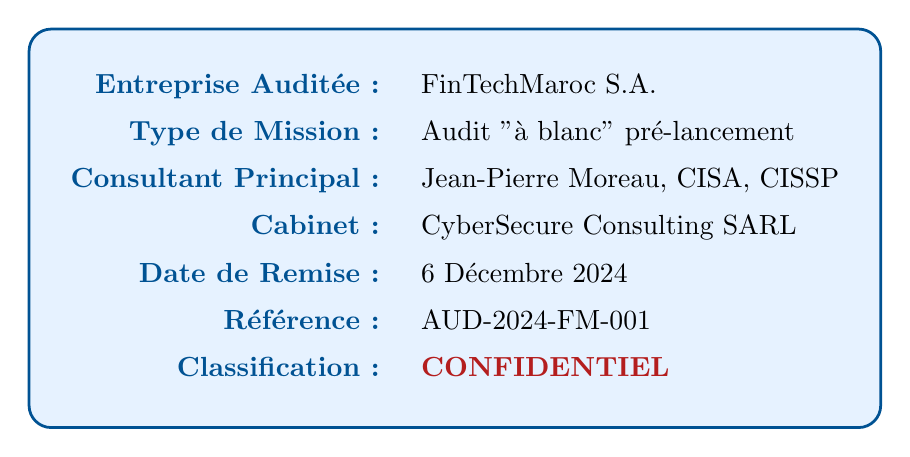
\begin{tikzpicture}
        \node[fill=lightblue,rounded corners=8pt,inner sep=15pt,draw=primaryblue,line width=1pt] {
            \begin{tabular}{@{}r@{\hspace{15pt}}l@{}}
                \textcolor{primaryblue}{\textbf{Entreprise Auditée :}} & FinTechMaroc S.A. \\[5pt]
                \textcolor{primaryblue}{\textbf{Type de Mission :}} & Audit "à blanc" pré-lancement \\[5pt]
                \textcolor{primaryblue}{\textbf{Consultant Principal :}} & Jean-Pierre Moreau, CISA, CISSP \\[5pt]
                \textcolor{primaryblue}{\textbf{Cabinet :}} & CyberSecure Consulting SARL \\[5pt]
                \textcolor{primaryblue}{\textbf{Date de Remise :}} & 6 Décembre 2024 \\[5pt]
                \textcolor{primaryblue}{\textbf{Référence :}} & AUD-2024-FM-001 \\[5pt]
                \textcolor{primaryblue}{\textbf{Classification :}} & \textcolor{criticalred}{\textbf{CONFIDENTIEL}}
            \end{tabular}
        };
    \end{tikzpicture}
    
    \vfill
    
    {\small\color{darkgray} 
        \textit{Ce document contient des informations confidentielles appartenant à FinTechMaroc S.A.}\\
        \textit{Toute reproduction ou diffusion non autorisée est strictement interdite.}
    }
    
    \vspace{1cm}
\end{center}
\end{titlepage}

% ================ DOCUMENT CONTROL ================
\thispagestyle{empty}
\section*{Contrôle du Document}

\begin{infobox}[Historique des Versions]
\begin{tabularx}{\textwidth}{|c|c|X|c|}
\hline
\rowcolor{tableheader}\textcolor{white}{\textbf{Version}} & \textcolor{white}{\textbf{Date}} & \textcolor{white}{\textbf{Modifications}} & \textcolor{white}{\textbf{Auteur}} \\
\hline
1.0 & 06/12/2024 & Version initiale complète (Phases 1-3) & J.P. Moreau \\
\hline
\end{tabularx}
\end{infobox}

\vspace{0.5cm}

\begin{infobox}[Distribution]
\begin{tabularx}{\textwidth}{|X|c|c|}
\hline
\rowcolor{tableheader}\textcolor{white}{\textbf{Destinataire}} & \textcolor{white}{\textbf{Fonction}} & \textcolor{white}{\textbf{Exemplaire}} \\
\hline
M. Ahmed Benali & Directeur Général, FinTechMaroc & Original \\
\hline
Mme Fatima Zeroual & Product Owner, PayMobile & Copie \\
\hline
M. Karim Idrissi & Lead Developer & Copie \\
\hline
Mme Sarah Martin & Responsable Conformité & Copie \\
\hline
\end{tabularx}
\end{infobox}

\vspace{0.5cm}

\begin{infobox}[Équipe d'Audit]
\begin{tabularx}{\textwidth}{|X|X|X|}
\hline
\rowcolor{tableheader}\textcolor{white}{\textbf{Nom}} & \textcolor{white}{\textbf{Rôle}} & \textcolor{white}{\textbf{Certifications}} \\
\hline
Jean-Pierre Moreau & Consultant Principal & CISA, CISSP, ISO 27001 LA \\
\hline
Marie Dubois & Analyste Sécurité & CEH, OSCP \\
\hline
Thomas Laurent & Expert PCI DSS & PCI QSA, PCIP \\
\hline
\end{tabularx}
\end{infobox}

\clearpage

% ================ TABLE OF CONTENTS ================
\tableofcontents
\clearpage

% ================ EXECUTIVE SUMMARY ================
\section{Résumé Exécutif}

\begin{execbox}
\begin{center}
{\Large\bfseries\color{primaryblue} Synthèse de l'Audit PayMobile}\\[0.5cm]
\end{center}

\textbf{\color{primaryblue}Objectif de la mission :} Évaluer la maturité des processus de développement et l'intégration des exigences de sécurité (Security by Design) pour le projet PayMobile avant son lancement prévu dans 6 mois.
\end{execbox}

\vspace{0.5cm}

% Risk Summary Dashboard
\begin{center}
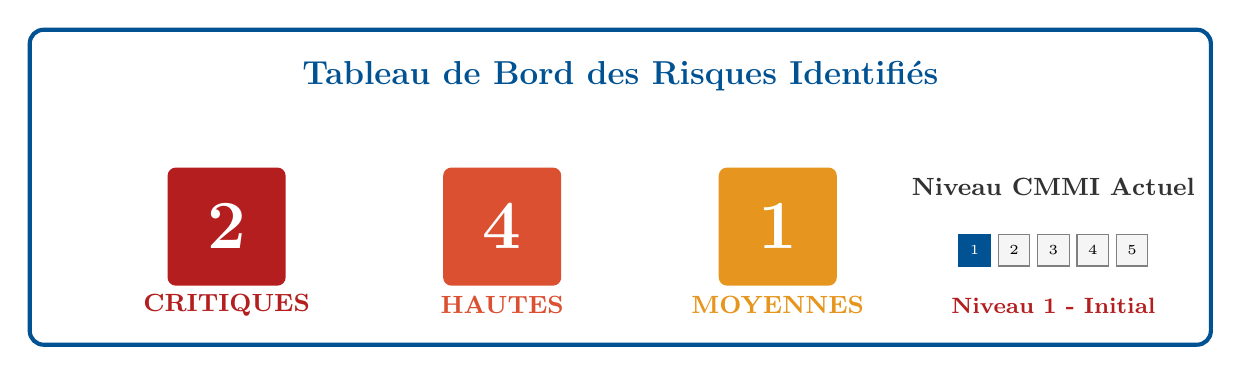
\begin{tikzpicture}
    % Main box
    \node[draw=primaryblue,line width=1.5pt,rounded corners=5pt,fill=white,minimum width=15cm,minimum height=4cm] (dashboard) {};
    
    % Title
    \node[anchor=north,font=\large\bfseries,color=primaryblue] at ([yshift=-0.3cm]dashboard.north) {Tableau de Bord des Risques Identifiés};
    
    % Risk counts
    \node[fill=criticalred,text=white,font=\Huge\bfseries,minimum size=1.5cm,rounded corners=3pt] at (-5,-0.5) {2};
    \node[font=\small\bfseries,color=criticalred] at (-5,-1.5) {CRITIQUES};
    
    \node[fill=highred,text=white,font=\Huge\bfseries,minimum size=1.5cm,rounded corners=3pt] at (-1.5,-0.5) {4};
    \node[font=\small\bfseries,color=highred] at (-1.5,-1.5) {HAUTES};
    
    \node[fill=mediumorange,text=white,font=\Huge\bfseries,minimum size=1.5cm,rounded corners=3pt] at (2,-0.5) {1};
    \node[font=\small\bfseries,color=mediumorange] at (2,-1.5) {MOYENNES};
    
    % CMMI Level
    \node[font=\small\bfseries,color=darkgray] at (5.5,0) {Niveau CMMI Actuel};
    \node at (5.5,-0.8) {\cmmilevel{1}};
    \node[font=\footnotesize,color=criticalred] at (5.5,-1.5) {\textbf{Niveau 1 - Initial}};
\end{tikzpicture}
\end{center}

\vspace{0.5cm}

% Main findings
\begin{criticalbox}[Constats Critiques]
\begin{itemize}[leftmargin=*,label=\textcolor{criticalred}{\ding{72}}]
    \item \textbf{US \#21 :} Mot de passe API stocké en clair dans un fichier de configuration — compromission système imminente
    \item \textbf{Absence totale de Security by Design :} Aucune User Story de sécurité formalisée dans le backlog
\end{itemize}
\end{criticalbox}

\vspace{0.3cm}

\begin{highbox}[Constats Majeurs]
\begin{itemize}[leftmargin=*,label=\textcolor{highred}{\ding{72}}]
    \item \textbf{US \#15 :} Stockage des 4 derniers chiffres de carte sans analyse PCI DSS appropriée
    \item \textbf{Plan de Test :} Absence totale de tests de sécurité (injection, XSS, robustesse)
    \item \textbf{Processus QA :} Auto-validation par les développeurs sans équipe QA indépendante
    \item \textbf{Conformité :} Méconnaissance des obligations PCI DSS par l'équipe projet
\end{itemize}
\end{highbox}

\vspace{0.3cm}

\begin{recobox}[Actions Prioritaires Immédiates]
\begin{enumerate}[leftmargin=*,label=\textcolor{lowgreen!80!black}{\textbf{\arabic*.}}]
    \item \textbf{J+15 :} Atelier d'urgence Security by Design avec toute l'équipe
    \item \textbf{J+30 :} Déploiement d'une solution de gestion des secrets (HashiCorp Vault)
    \item \textbf{J+30 :} Analyse d'impact PCI DSS avec expert conformité
    \item \textbf{J+60 :} Intégration des tests de sécurité automatisés dans la CI/CD
\end{enumerate}
\end{recobox}

\clearpage

% ================ PHASE 1: INTRODUCTION ================
\section{Introduction et Contexte (Phase 1)}

\subsection{Contexte Général du Projet}

\begin{infobox}[Présentation PayMobile]
\textbf{FinTechMaroc S.A.} développe l'application mobile \textbf{PayMobile}, une solution de paiement innovante destinée aux petits commerçants marocains. Cette application permettra :

\begin{multicols}{2}
\begin{itemize}[leftmargin=*]
    \item Acceptation des paiements par carte
    \item Saisie manuelle des informations de carte
    \item Consultation de l'historique des transactions
    \item Génération de reçus électroniques
    \item Tableau de bord des ventes
    \item Notifications en temps réel
\end{itemize}
\end{multicols}

\textbf{Échéance MVP :} 6 mois | \textbf{Budget :} Non communiqué | \textbf{Équipe :} 8 personnes
\end{infobox}

\vspace{0.3cm}

\subsection{Enjeux Critiques}

\begin{center}
\begin{tikzpicture}
    \node[draw=criticalred,line width=1.5pt,fill=criticalred!5,rounded corners=5pt,text width=14cm,align=center,inner sep=10pt] {
        \textcolor{criticalred}{\Large\faExclamationTriangle\quad\textbf{ATTENTION}\quad\faExclamationTriangle}\\[0.3cm]
        \textcolor{darkgray}{Le projet PayMobile manipule des \textbf{données de paiement sensibles} (numéros de carte, transactions).\\
        La conformité \textbf{PCI DSS} est \textbf{obligatoire} et non négociable pour tout système manipulant ces données.\\[0.2cm]
        \textit{Tout manquement expose FinTechMaroc à des sanctions financières, blocage des prestataires de paiement, et atteinte irréversible à la réputation.}}
    };
\end{tikzpicture}
\end{center}

\subsection{Objectifs de l'Audit}

\begin{center}
\begin{tabularx}{0.95\textwidth}{|c|X|c|}
\hline
\rowcolor{tableheader}\textcolor{white}{\textbf{\#}} & \textcolor{white}{\textbf{Objectif}} & \textcolor{white}{\textbf{Statut}} \\
\hline
\rowcolor{tablerow1}1 & Évaluer la maturité des processus de développement selon le modèle CMMI & \statusfail \\
\hline
\rowcolor{tablerow2}2 & Vérifier l'intégration des principes de Security by Design & \statusfail \\
\hline
\rowcolor{tablerow1}3 & Évaluer la préparation pour les tests, la validation et la conformité PCI DSS & \statusfail \\
\hline
\rowcolor{tablerow2}4 & Proposer un plan d'amélioration priorisé et actionnable & \statusok \\
\hline
\end{tabularx}
\end{center}

\subsection{Périmètre de l'Audit}

\begin{center}
\begin{tikzpicture}
    % Included box
    \node[draw=lowgreen,line width=1.5pt,fill=lowgreen!5,rounded corners=5pt,text width=6.5cm,align=left,inner sep=10pt] (included) at (-4,0) {
        \textcolor{lowgreen}{\large\faCheckCircle\quad\textbf{INCLUS}}\\[0.3cm]
        \textcolor{darkgray}{
        \ding{51} Gestion des exigences\\
        \ding{51} Documentation projet\\
        \ding{51} Organisation et processus\\
        \ding{51} Plan de test\\
        \ding{51} Interviews équipe\\
        \ding{51} Analyse des User Stories}
    };
    
    % Excluded box
    \node[draw=criticalred,line width=1.5pt,fill=criticalred!5,rounded corners=5pt,text width=6.5cm,align=left,inner sep=10pt] (excluded) at (4,0) {
        \textcolor{criticalred}{\large\faTimesCircle\quad\textbf{EXCLUS}}\\[0.3cm]
        \textcolor{darkgray}{
        \ding{55} Audit du code source\\
        \ding{55} Tests d'intrusion\\
        \ding{55} Audit financier\\
        \ding{55} Revue d'infrastructure\\
        \ding{55} Tests de charge\\
        \ding{55} Évaluation RH}
    };
\end{tikzpicture}
\end{center}

\clearpage

% ================ APPROACH & CRITERIA ================
\section{Approche et Critères d'Audit}

\subsection{Référentiels Utilisés}

\begin{center}
\begin{tikzpicture}
    % CMMI Box
    \node[draw=primaryblue,line width=1.5pt,fill=lightblue,rounded corners=8pt,text width=4.5cm,align=center,inner sep=10pt] (cmmi) at (-5.5,0) {
        \textcolor{primaryblue}{\Large\faCogs}\\[0.2cm]
        \textcolor{primaryblue}{\large\textbf{CMMI}}\\[0.2cm]
        \textcolor{darkgray}{\small Capability Maturity Model Integration\\[0.1cm]
        \textit{Évaluation de la maturité des processus}}
    };
    
    % PCI DSS Box
    \node[draw=primaryblue,line width=1.5pt,fill=lightblue,rounded corners=8pt,text width=4.5cm,align=center,inner sep=10pt] (pci) at (0,0) {
        \textcolor{primaryblue}{\Large\faCreditCard}\\[0.2cm]
        \textcolor{primaryblue}{\large\textbf{PCI DSS v4.0}}\\[0.2cm]
        \textcolor{darkgray}{\small Payment Card Industry Data Security Standard\\[0.1cm]
        \textit{Sécurité données de paiement}}
    };
    
    % OWASP Box
    \node[draw=primaryblue,line width=1.5pt,fill=lightblue,rounded corners=8pt,text width=4.5cm,align=center,inner sep=10pt] (owasp) at (5.5,0) {
        \textcolor{primaryblue}{\Large\faMobileAlt}\\[0.2cm]
        \textcolor{primaryblue}{\large\textbf{OWASP}}\\[0.2cm]
        \textcolor{darkgray}{\small Mobile Top 10 2024\\[0.1cm]
        \textit{Bonnes pratiques sécurité mobile}}
    };
\end{tikzpicture}
\end{center}

\vspace{0.5cm}

\subsection{Critères d'Évaluation}

\begin{center}
\begin{tabularx}{0.95\textwidth}{|>{\centering\arraybackslash}p{0.5cm}|X|>{\centering\arraybackslash}p{2cm}|}
\hline
\rowcolor{tableheader}\textcolor{white}{\textbf{\#}} & \textcolor{white}{\textbf{Critère d'Évaluation}} & \textcolor{white}{\textbf{Résultat}} \\
\hline
\rowcolor{tablerow1}C1 & \textbf{Security by Design} — Intégration de la sécurité dès la conception & \statusfail Non conforme \\
\hline
\rowcolor{tablerow2}C2 & \textbf{Protection des données sensibles} — Chiffrement, masquage, contrôle d'accès & \statusfail Non conforme \\
\hline
\rowcolor{tablerow1}C3 & \textbf{Gestion des secrets} — Stockage sécurisé des credentials et clés API & \statusfail Non conforme \\
\hline
\rowcolor{tablerow2}C4 & \textbf{Couverture des tests} — Tests fonctionnels, sécurité et robustesse & \statusfail Non conforme \\
\hline
\rowcolor{tablerow1}C5 & \textbf{Indépendance de validation} — Séparation développement/QA & \statusfail Non conforme \\
\hline
\rowcolor{tablerow2}C6 & \textbf{Conformité réglementaire} — Maîtrise des obligations PCI DSS & \statusfail Non conforme \\
\hline
\end{tabularx}
\end{center}

\subsection{Documents Analysés}

\begin{infobox}[Sources de Preuves]
\begin{tabularx}{\textwidth}{|c|X|c|}
\hline
\rowcolor{tableheader}\textcolor{white}{\textbf{Réf.}} & \textcolor{white}{\textbf{Document}} & \textcolor{white}{\textbf{Date}} \\
\hline
Doc 1 & Backlog PayMobile — User Stories v2.3 & 15/11/2024 \\
\hline
Doc 2 & Plan de Test PayMobile — CT-01 à CT-04 & 20/11/2024 \\
\hline
Doc 3 & Compte-rendu interviews (PO, Lead Dev) & 28/11/2024 \\
\hline
Doc 4 & Architecture technique (draft) & 10/11/2024 \\
\hline
\end{tabularx}
\end{infobox}

\clearpage

% ================ PHASE 2: FINDINGS ================
\section{Constats et Analyse des Preuves (Phase 2)}

\subsection{Analyse des Exigences et Security by Design}

\begin{center}
\renewcommand{\arraystretch}{1.4}
\begin{tabularx}{\textwidth}{|>{\centering\arraybackslash}p{1.8cm}|X|>{\centering\arraybackslash}p{2.2cm}|>{\centering\arraybackslash}p{1.5cm}|}
\hline
\rowcolor{tableheader}\textcolor{white}{\textbf{User Story}} & \textcolor{white}{\textbf{Analyse et Risque Identifié}} & \textcolor{white}{\textbf{Critère}} & \textcolor{white}{\textbf{Preuve}} \\
\hline
\rowcolor{tablerow1}
\textbf{US \#12} & \textbf{Saisie manuelle des informations de carte}\\
Risque d'exposition des données PAN en mémoire et logs. Augmentation significative du périmètre PCI DSS (SAQ D au lieu de SAQ P2PE). & C2 & Doc 1 \\
\hline
\rowcolor{tablerow2}
\cellcolor{criticalred!15}\textbf{US \#15} & \cellcolor{criticalred!15}\textbf{Affichage des 4 derniers chiffres}\\
Consultation des 100 dernières transactions incluant les 4 derniers chiffres de carte. Nécessite des mesures strictes de stockage et d'accès (PCI DSS Req. 3.4). & \cellcolor{criticalred!15}C2 + C6 & \cellcolor{criticalred!15}Doc 1 \\
\hline
\rowcolor{tablerow1}
\cellcolor{criticalred!30}\textbf{US \#21} & \cellcolor{criticalred!30}\textbf{\textcolor{criticalred}{CRITIQUE :} Mot de passe API en clair}\\
Secret API stocké en clair dans \texttt{config.properties}. Compromission immédiate en cas d'accès au dépôt ou serveur. Violation PCI DSS Req. 8.3.2. & \cellcolor{criticalred!30}C3 & \cellcolor{criticalred!30}Doc 1 \\
\hline
\rowcolor{tablerow2}
\cellcolor{criticalred!30}\textbf{Général} & \cellcolor{criticalred!30}\textbf{\textcolor{criticalred}{CRITIQUE :} Absence de Security by Design}\\
Aucune User Story de sécurité ou non-fonctionnelle dans le backlog. La sécurité n'est pas considérée comme un livrable. & \cellcolor{criticalred!30}C1 & \cellcolor{criticalred!30}Doc 1, Doc 3 \\
\hline
\end{tabularx}
\end{center}

\vspace{0.5cm}

\subsection{Analyse du Plan de Test et de la Maturité}

\begin{center}
\renewcommand{\arraystretch}{1.4}
\begin{tabularx}{\textwidth}{|>{\centering\arraybackslash}p{2.2cm}|X|>{\centering\arraybackslash}p{2.2cm}|>{\centering\arraybackslash}p{1.5cm}|}
\hline
\rowcolor{tableheader}\textcolor{white}{\textbf{Élément}} & \textcolor{white}{\textbf{Analyse et Lacunes}} & \textcolor{white}{\textbf{Critère}} & \textcolor{white}{\textbf{Preuve}} \\
\hline
\rowcolor{tablerow1}
\textbf{Plan de Test}\\(CT-01 à CT-04) & Tests centrés exclusivement sur les scénarios nominaux. \textbf{Absence totale} de tests de sécurité : injection SQL, XSS, tests de robustesse, validation des entrées. & C4 & Doc 2 \\
\hline
\rowcolor{tablerow2}
\textbf{Processus QA} & Auto-validation par les développeurs eux-mêmes. Pas d'équipe QA indépendante ni de processus formel de revue. Biais de confirmation inévitable. & C5 & Doc 3 \\
\hline
\rowcolor{tablerow1}
\textbf{Vision PO} & \textit{"La sécurité, on l'ajoutera plus tard, après le MVP"} — La sécurité est perçue comme optionnelle et non comme une exigence fondamentale. & C1 + C6 & Doc 3 \\
\hline
\rowcolor{tablerow2}
\textbf{Maturité CMMI} & Processus ad hoc, non documentés, dépendants des individus. Aucune mesure, aucun indicateur de performance. Caractéristique du \textbf{Niveau 1 (Initial)}. & Tous & Doc 1-3 \\
\hline
\end{tabularx}
\end{center}

\clearpage

\subsection{Constats Majeurs Détaillés}

% Constat 1
\begin{criticalbox}[\faExclamationTriangle\quad Constat Majeur 1 : Absence de Security by Design et Gestion des Secrets]
\begin{tabularx}{\textwidth}{@{}r@{\hspace{10pt}}X@{}}
\textbf{Priorité :} & \criticalrisk \\[0.3cm]
\textbf{Description :} & Le projet ne dispose d'aucune exigence de sécurité formalisée. Plus grave, le mot de passe de l'API de paiement est stocké en clair dans un fichier de configuration versionné. \\[0.3cm]
\textbf{Risque :} & Compromission totale des systèmes de paiement, transactions frauduleuses, vol de données clients, responsabilité légale de FinTechMaroc, perte de la certification PCI et blocage par les processeurs de paiement. \\[0.3cm]
\textbf{Cause Racine :} & Pression sur le MVP, absence de culture sécurité, manque de sensibilisation de l'équipe aux enjeux PCI DSS. \\[0.3cm]
\textbf{Preuves :} & US \#21 (Doc 1), Déclarations du PO (Doc 3), Fichier \texttt{config.properties} \\
\end{tabularx}
\end{criticalbox}

\vspace{0.4cm}

% Constat 2
\begin{highbox}[\faExclamationCircle\quad Constat Majeur 2 : Couverture Tests Insuffisante et Absence d'Indépendance]
\begin{tabularx}{\textwidth}{@{}r@{\hspace{10pt}}X@{}}
\textbf{Priorité :} & \highrisk \\[0.3cm]
\textbf{Description :} & Le plan de test ne couvre que les scénarios fonctionnels nominaux. Aucun test de sécurité, de robustesse ou de validation des entrées n'est prévu. Les développeurs valident leur propre code. \\[0.3cm]
\textbf{Risque :} & Vulnérabilités non détectées déployées en production (injection SQL, XSS, buffer overflow), régressions silencieuses, incidents de sécurité post-lancement. \\[0.3cm]
\textbf{Cause Racine :} & Absence de rôle QA dédié, tests perçus comme une charge plutôt qu'un investissement, processus informels. \\[0.3cm]
\textbf{Preuves :} & Doc 2 (Plan de test), Propos du Lead Dev (Doc 3) \\
\end{tabularx}
\end{highbox}

\vspace{0.4cm}

% Constat 3
\begin{highbox}[\faExclamationCircle\quad Constat Majeur 3 : Non-Maîtrise des Obligations PCI DSS]
\begin{tabularx}{\textwidth}{@{}r@{\hspace{10pt}}X@{}}
\textbf{Priorité :} & \highrisk \\[0.3cm]
\textbf{Description :} & L'équipe projet (PO et Lead Dev) n'a pas connaissance des exigences PCI DSS applicables. Aucune analyse d'impact réglementaire n'a été réalisée. Le stockage des 4 derniers chiffres est implémenté sans mesures de protection adéquates. \\[0.3cm]
\textbf{Risque :} & Non-conformité PCI DSS entraînant l'impossibilité de traiter des paiements, amendes pouvant atteindre 100 000\$/mois, atteinte irréversible à la réputation, responsabilité en cas de breach. \\[0.3cm]
\textbf{Cause Racine :} & Absence d'expertise conformité dans l'équipe, pas de budget alloué à la formation réglementaire. \\[0.3cm]
\textbf{Preuves :} & US \#15 (Doc 1), Déclarations du PO (Doc 3) \\
\end{tabularx}
\end{highbox}

\clearpage

% ================ PHASE 3: RECOMMENDATIONS ================
\section{Conclusion et Recommandations Stratégiques (Phase 3)}

\subsection{Conclusion Générale}

\begin{center}
\begin{tikzpicture}
    \node[draw=criticalred,line width=2pt,fill=criticalred!5,rounded corners=8pt,text width=14cm,align=center,inner sep=15pt] {
        \textcolor{criticalred}{\Huge\faExclamationTriangle}\\[0.3cm]
        {\Large\bfseries\color{criticalred} VERDICT : NON-CONFORMITÉ CRITIQUE}\\[0.4cm]
        \textcolor{darkgray}{\large Le projet PayMobile présente un \textbf{niveau de maturité insuffisant} (CMMI Niveau 1).\\[0.2cm]
        La sécurité et la conformité PCI DSS \textbf{ne sont pas intégrées} dès la conception.\\[0.2cm]
        \textbf{Le MVP ne peut pas être lancé en l'état} sans exposer FinTechMaroc\\à des risques légaux, financiers et réputationnels majeurs.}
    };
\end{tikzpicture}
\end{center}

\vspace{0.5cm}

\subsection{Plan de Recommandations Priorisé}

\begin{center}
\renewcommand{\arraystretch}{1.5}
\begin{tabularx}{\textwidth}{|>{\centering\arraybackslash}p{1.2cm}|X|>{\centering\arraybackslash}p{1.8cm}|>{\centering\arraybackslash}p{1.8cm}|>{\centering\arraybackslash}p{2cm}|}
\hline
\rowcolor{tableheader}\textcolor{white}{\textbf{Réf.}} & \textcolor{white}{\textbf{Recommandation}} & \textcolor{white}{\textbf{Priorité}} & \textcolor{white}{\textbf{Délai}} & \textcolor{white}{\textbf{Responsable}} \\
\hline
\rowcolor{criticalred!10}
\textbf{R1a} & \textbf{Atelier d'urgence Security by Design}\\Définir les exigences non-fonctionnelles critiques (chiffrement, sessions, gestion des erreurs). Utiliser OWASP Mobile Top 10 comme référence. & \criticalrisk & 15 jours & PO + Lead Dev \\
\hline
\rowcolor{criticalred!10}
\textbf{R1b} & \textbf{Gestion sécurisée des secrets}\\Déployer HashiCorp Vault ou Azure Key Vault. Supprimer IMMÉDIATEMENT tous les secrets en clair. Rotation des credentials compromis. & \criticalrisk & 1 mois & Lead Dev + Ops \\
\hline
\rowcolor{highred!10}
\textbf{R1c} & \textbf{Revue des User Stories}\\Intégrer des critères d'acceptation sécurité pour chaque US (validation entrées, logging sécurisé, masquage données). & \highrisk & 3 sem. & PO \\
\hline
\rowcolor{highred!10}
\textbf{R2a} & \textbf{Intégration tests de sécurité}\\Ajouter cas de test : injection SQL, XSS, CSRF, validation entrées. Intégrer SAST/DAST dans pipeline CI/CD. & \highrisk & 2 mois & Lead Dev + QA \\
\hline
\rowcolor{highred!10}
\textbf{R2b} & \textbf{Créer fonction QA indépendante}\\Recruter ou nommer un responsable QA. Objectif : atteindre CMMI Niveau 2. & \highrisk & 2 mois & Direction \\
\hline
\rowcolor{highred!10}
\textbf{R3a} & \textbf{Analyse d'impact PCI DSS}\\Mission flash avec un QSA pour déterminer le SAQ applicable et les obligations exactes. & \highrisk & 1 mois & Direction \\
\hline
\rowcolor{mediumorange!10}
\textbf{R3b} & \textbf{Formation obligatoire PCI DSS}\\Former PO, Lead Dev et équipe sur les fondamentaux PCI DSS et OWASP. & \mediumrisk & 3 mois & RH + Direction \\
\hline
\end{tabularx}
\end{center}

\clearpage

\subsection{Feuille de Route 30 Jours}

\begin{center}
\begin{tikzpicture}[
    milestone/.style={draw=primaryblue,line width=1.5pt,fill=lightblue,rounded corners=5pt,text width=11cm,align=left,inner sep=10pt},
    arrow/.style={->,>=stealth,line width=2pt,primaryblue}
]
    % J+3
    \node[milestone] (j3) at (0,0) {
        \textcolor{primaryblue}{\large\faCalendarAlt\quad\textbf{J+3 : Lancement}}\\[0.2cm]
        \textcolor{darkgray}{
        \ding{51} Réunion de lancement avec Direction et équipe projet\\
        \ding{51} Préparation de l'atelier Security by Design\\
        \ding{51} Collecte des spécifications critiques\\
        \ding{51} Identification des ressources nécessaires}
    };
    
    % J+10
    \node[milestone] (j10) at (0,-3.5) {
        \textcolor{primaryblue}{\large\faCalendarAlt\quad\textbf{J+10 : Premières Actions}}\\[0.2cm]
        \textcolor{darkgray}{
        \ding{51} Mise à jour initiale des User Stories avec critères sécurité\\
        \ding{51} Suppression des secrets en clair du dépôt\\
        \ding{51} Contact avec prestataire Key Vault\\
        \ding{51} Identification d'un expert PCI DSS}
    };
    
    % J+15
    \node[milestone] (j15) at (0,-7) {
        \textcolor{secondaryblue}{\large\faCalendarAlt\quad\textbf{J+15 : Atelier Security by Design}}\\[0.2cm]
        \textcolor{darkgray}{
        \ding{51} Atelier d'une journée avec toute l'équipe\\
        \ding{51} Définition des exigences non-fonctionnelles\\
        \ding{51} Priorisation des corrections critiques\\
        \ding{51} Validation du plan d'action par la Direction}
    };
    
    % J+30
    \node[milestone] (j30) at (0,-10.5) {
        \textcolor{lowgreen!80!black}{\large\faCalendarAlt\quad\textbf{J+30 : Premiers Livrables}}\\[0.2cm]
        \textcolor{darkgray}{
        \ding{51} Solution de gestion des secrets opérationnelle\\
        \ding{51} Plan de test révisé avec cas de sécurité\\
        \ding{51} Rapport d'analyse PCI DSS reçu\\
        \ding{51} Roadmap QA formalisée}
    };
    
    % Arrows
    \draw[arrow] (j3.south) -- (j10.north);
    \draw[arrow] (j10.south) -- (j15.north);
    \draw[arrow] (j15.south) -- (j30.north);
\end{tikzpicture}
\end{center}

\clearpage

\subsection{Annexes et Ressources}

\begin{infobox}[A. Modèle User Story avec Critères Sécurité]
\textbf{Format recommandé :}\\[0.3cm]
\texttt{En tant que [rôle], je veux [fonctionnalité] afin de [bénéfice].}\\[0.3cm]
\textbf{Critères d'acceptation sécurité obligatoires :}
\begin{itemize}[leftmargin=*]
    \item[\ding{51}] Toutes les entrées utilisateur sont validées côté serveur
    \item[\ding{51}] Les données sensibles sont chiffrées au repos et en transit (AES-256, TLS 1.3)
    \item[\ding{51}] Les erreurs ne révèlent pas d'information système
    \item[\ding{51}] Les actions sont tracées dans un log sécurisé
    \item[\ding{51}] Les données de carte sont masquées (affichage **** **** **** 1234)
\end{itemize}
\end{infobox}

\vspace{0.4cm}

\begin{infobox}[B. Checklist PCI DSS Minimale — Stockage des 4 Derniers Chiffres]
\begin{tabularx}{\textwidth}{|>{\centering\arraybackslash}p{1.5cm}|X|>{\centering\arraybackslash}p{2cm}|}
\hline
\rowcolor{tableheader}\textcolor{white}{\textbf{Req.}} & \textcolor{white}{\textbf{Exigence}} & \textcolor{white}{\textbf{Statut}} \\
\hline
3.4 & Rendre le PAN illisible partout où il est stocké & \statusfail À vérifier \\
\hline
3.5 & Protéger les clés de chiffrement & \statusfail À implémenter \\
\hline
7.1 & Limiter l'accès aux données de titulaires de cartes & \statusfail À définir \\
\hline
8.3 & Sécuriser l'authentification pour accès aux données & \statusfail À implémenter \\
\hline
10.1 & Implémenter des pistes d'audit & \statusfail À implémenter \\
\hline
\end{tabularx}
\end{infobox}

\vspace{0.4cm}

\begin{infobox}[C. Template Plan de Test — Sections Sécurité]
\textbf{Sections obligatoires à ajouter :}
\begin{multicols}{2}
\begin{itemize}[leftmargin=*]
    \item Tests d'injection SQL
    \item Tests XSS (réfléchi et stocké)
    \item Tests CSRF
    \item Validation des entrées
    \item Tests de session (timeout, fixation)
    \item Tests d'authentification
    \item Tests d'autorisation
    \item Tests de robustesse (fuzzing)
    \item Tests de chiffrement
    \item Tests de logging sécurisé
\end{itemize}
\end{multicols}
\end{infobox}

\clearpage

% ================ FINAL CONCLUSION ================
\section{Conclusion Finale}

\begin{center}
\begin{tikzpicture}
    \node[draw=primaryblue,line width=2pt,fill=lightblue,rounded corners=10pt,text width=14cm,align=center,inner sep=20pt] {
        {\Huge\color{primaryblue}\faShieldAlt}\\[0.5cm]
        {\Large\bfseries\color{primaryblue} Message Clé}\\[0.5cm]
        \textcolor{darkgray}{\large L'adoption rapide des recommandations critiques\\(\textbf{R1a}, \textbf{R1b}, \textbf{R3a}, \textbf{R2a}) est \textbf{indispensable}\\pour garantir un lancement MVP sûr et conforme.\\[0.3cm]
        La crédibilité de FinTechMaroc lors de la prochaine levée de fonds\\dépend directement de la maturité sécurité démontrée.\\[0.5cm]
        \textit{La sécurité n'est pas un coût — c'est un investissement\\qui protège votre business et vos clients.}}
    };
\end{tikzpicture}
\end{center}

\vspace{1.5cm}

% Contact box
\begin{center}
\begin{tikzpicture}
    \node[draw=accentgold,line width=1.5pt,fill=accentgold!5,rounded corners=8pt,text width=12cm,align=center,inner sep=15pt] {
        {\Large\bfseries\color{primaryblue} Contact Équipe d'Audit}\\[0.5cm]
        \begin{tabular}{@{}cl@{}}
            \textcolor{primaryblue}{\faUser} & \textbf{Jean-Pierre Moreau}, CISA, CISSP \\[0.2cm]
            \textcolor{primaryblue}{\faBuilding} & CyberSecure Consulting SARL \\[0.2cm]
            \textcolor{primaryblue}{\faEnvelope} & \href{mailto:jp.moreau@cybersecure-consulting.ma}{jp.moreau@cybersecure-consulting.ma} \\[0.2cm]
            \textcolor{primaryblue}{\faPhone} & +212 5 22 XX XX XX \\[0.2cm]
            \textcolor{primaryblue}{\faGlobe} & \href{https://www.cybersecure-consulting.ma}{www.cybersecure-consulting.ma} \\
        \end{tabular}
    };
\end{tikzpicture}
\end{center}

\vspace{1cm}

\begin{center}
\textcolor{darkgray}{\rule{0.6\textwidth}{0.5pt}}\\[0.5cm]
{\small\color{darkgray}\textit{Ce rapport a été préparé avec le plus grand soin et selon les standards professionnels.\\
Les conclusions et recommandations sont basées sur les informations fournies au moment de l'audit.\\
CyberSecure Consulting ne peut être tenu responsable des décisions prises sur la base de ce rapport.}}\\[0.5cm]
{\footnotesize\color{darkgray}\textbf{Référence :} AUD-2024-FM-001 | \textbf{Classification :} CONFIDENTIEL | \textbf{Date :} 6 Décembre 2024}
\end{center}

\end{document}



